\documentclass{beamer}
\usepackage{amssymb, amsfonts, latexsym, amsthm, amsmath, framed, esvect, parskip}
\usepackage{amsmath, amssymb, framed, tcolorbox, mathrsfs, xcolor, graphicx}
\usepackage{multirow,booktabs, makecell}
\usepackage[backend=biber,style=numeric,sorting=none]{biblatex}
\setbeamerfont{footnote}{size=\tiny}
\addbibresource{ref.bib}
\tcbuselibrary{theorems}
\usepackage{listings}
\definecolor{green}{rgb}{0,0.6,0}
\definecolor{gray}{rgb}{0.5,0.5,0.5}
\definecolor{mauve}{rgb}{0.58,0,0.82}
\lstset{
    frame=none,
    language=Java,
    showstringspaces=false,
    columns=fullflexible,
    basicstyle = \ttfamily\small,
    numbers=none,
    numberstyle=\tiny\color{gray},
    keywordstyle=\color{blue},
    commentstyle=\color{green},
    stringstyle=\color{mauve},
    breaklines=true,
    morekeywords={function},
    breakatwhitespace=true,
    tabsize=4
}

% Beamer theme setting
\definecolor{myteal}{cmyk}{0.5,0,0.15,0}
\usecolortheme[named=myteal]{structure}
\definecolor{my-yellow}{cmyk}{0,0.2,0.7,0,1.00}
\definecolor{my-blue}{cmyk}{0.80, 0.13, 0.14, 0.04, 1.00}
\definecolor{my-green}{cmyk}{0.4,0,0.4,0,1.00}
\tcbset{
defstyle/.style={fonttitle=\bfseries\upshape, colback=my-yellow!5,colframe=my-yellow!80!black},
theostyle/.style={fonttitle=\bfseries\upshape, colback=my-blue!5,colframe=my-blue!80!black},
corstyle/.style={fonttitle=\bfseries\upshape, colback=my-green!5,colframe=my-green!80!black},
}
\usetheme{Madrid}
\setbeamertemplate{itemize items}[triangle]
\setbeamertemplate{enumerate items}[default]

\title{Week 2 Report}
\author{Ben Chen}
\institute{Dept of Computer Science and Engineering, SUSTech}
\date{\today}

\begin{document}
\frame{\titlepage}

\begin{frame}{TOC}
\begin{table}[ht]
    \tiny
	\centering
	\begin{tabular}[c]{ccccc}
		\toprule
        Title & Conference & Institute & Authors & Idea \\
		\midrule
        \makecell{A Security RISC: \\ Microarchitectural Attacks \\ on Hardware RISC-V CPUs} & Oakland '23 & CISPA & \makecell{Lukas Gerlach\\ Daniel Weber\\ Ruiyi Zhang\\ Michael Schwarz}  & \makecell{Cache+Time, Flush+Fault, CycleDrift \\ on SiFive U74 \& T-Head C906 \\ with 6 case studies} \\ \\ 
        \makecell{(M)WAIT for It: \\ Bridging the Gap between \\ Microarchitectural and \\ Architectural Side Channels} & USENIX '23 & CISPA & \makecell{Ruiyi Zhang\\ Taehyun Kim\\ Daniel Weber\\Michael Schwarz} & \makecell{Exploiting \texttt{umonitor} and \texttt{umwait} \\ to enhance spectre attack \\ without timer} \\
		\bottomrule
	\end{tabular}
\end{table}
\end{frame}

\begin{frame}{A Security RISC\cite{a-secure-risc}}
Systematic analysis of microarchitectural components:
\begin{itemize}[<+->]
    \item Hardware Timer: \texttt{rdcycle} and \texttt{rdtime} instructions on both CPUs, a higher resolution in retire instruction counter on U74 via \texttt{rdinstret} or \texttt{csrr} instructions.
    \item Cache: Capacity and replacement policy (deterministic), FIFO on C906 and PLRU on U74; Cache maintainance instructions: \texttt{fence.i} by ISA and \texttt{dcache.civa} by C906 $\Rightarrow$ efficient cache eviction.
    \item TLB: SV39, two separate 10-entry fully-associative TLBs for data and instructions, effectively evictable.
    \item BRU: In-order pipeline but speculative prefetching, with BHT, BJT, and RAS.
\end{itemize}
\end{frame}

\begin{frame}{A Security RISC\cite{a-secure-risc}}
\begin{figure}[ht]
    \begin{center}
    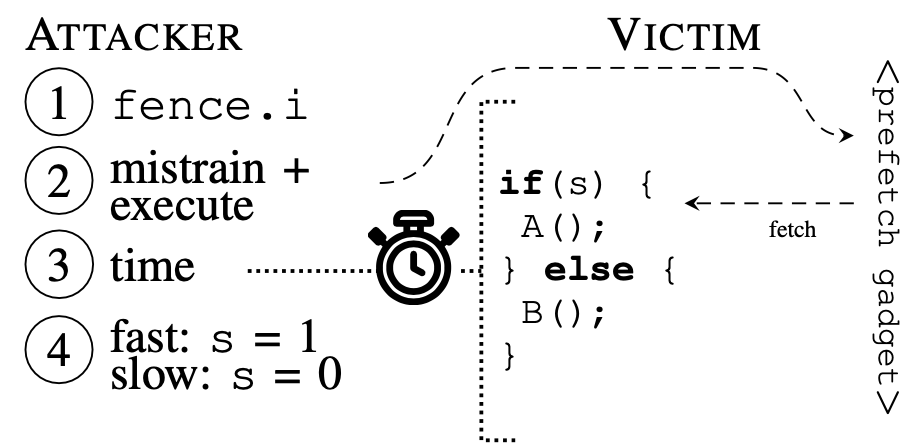
\includegraphics[width=0.7\textwidth]{img/cache-time.png}
    \end{center}
\end{figure}
\begin{center}
flush i\$ $\Rightarrow$ mistrain to load \texttt{A} but not \texttt{B} $\Rightarrow$ timing difference
\end{center}
\end{frame}

\begin{frame}{A Security RISC\cite{a-secure-risc}}
\begin{figure}[ht]
    \begin{center}
    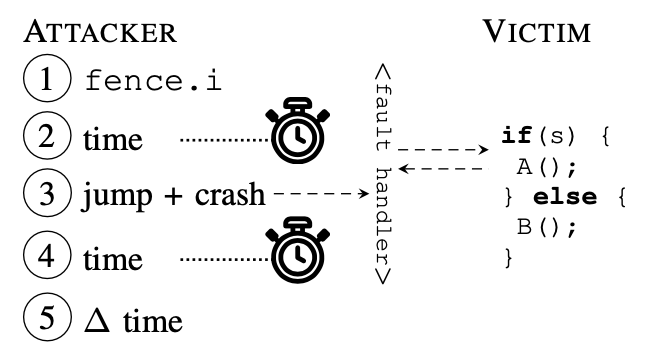
\includegraphics[width=0.7\textwidth]{img/flush-fault.png}
    \end{center}
\end{figure}
\begin{center}
    flush i\$ $\Rightarrow$ jump to victim's code and trigger a fault $\Rightarrow$ timing difference to determine whether \texttt{A} or \texttt{B} is in cache 
    \begin{itemize}
        \item \texttt{addi a0, zero, zero} in attacker's code
        \item then jump to \texttt{ld xx, 0(a0)} in victim's code
    \end{itemize}
\end{center}
\end{frame}

\begin{frame}{A Security RISC\cite{a-secure-risc}}
Monitor number of retired instructions with a certain cycles:
\begin{table}[ht]
    \tiny
	\centering
	\begin{tabular}[c]{cccc}
		\toprule
        Platform & \texttt{SBI\_EXT\_BASE\_GET\_MVENDORID} & \texttt{SBI\_EXT\_0\_1\_CONSOLE\_PUTCHAR} & padded square-and-multiply\\
		\midrule
        U74 & 963 cycles & 85507 cycles & 14(-3) instructions \\ 
        C906 & 613 cycles & 85109 cycles & 18(-2) instructions \\ 
		\bottomrule
	\end{tabular}
\end{table}
\end{frame}

\begin{frame}{A Security RISC\cite{a-secure-risc}}
Case studies:
\begin{itemize}[<+->]
    \item Square and Multiply in MbedTLS: Flush+Fault, Cache+Time
    \item Breaking KASLR: CycleDrift, timming difference in page-table walk
    \item Zigzagger Bypass: CycleDrift
    \item Leaking Contents of a Drop-Box Folder: CycleDrift,
    \item Interrupt Detection: CycleDrift
    \item OpenSSL 1.0.1 AES T-Table: Cache attacks
\end{itemize}
\end{frame}

\begin{frame}{(M)WAIT For it\cite{mwait}}
Motivation:
\begin{itemize}[<+->]
    \item Intel introduces \texttt{umonitor} and \texttt{umwait} in Alder Lake to optimize idle-loop.
    \item AMD has similar instructions \texttt{monitorx} and \texttt{mwaitx}.
    \item \texttt{umonitor} tells monitor component to start monitoring a memory region, \texttt{umwait} waits until the region is modified (either in cache or memory), interrupt arrives or a timeout.
\end{itemize}
\begin{figure}
    \begin{center}
    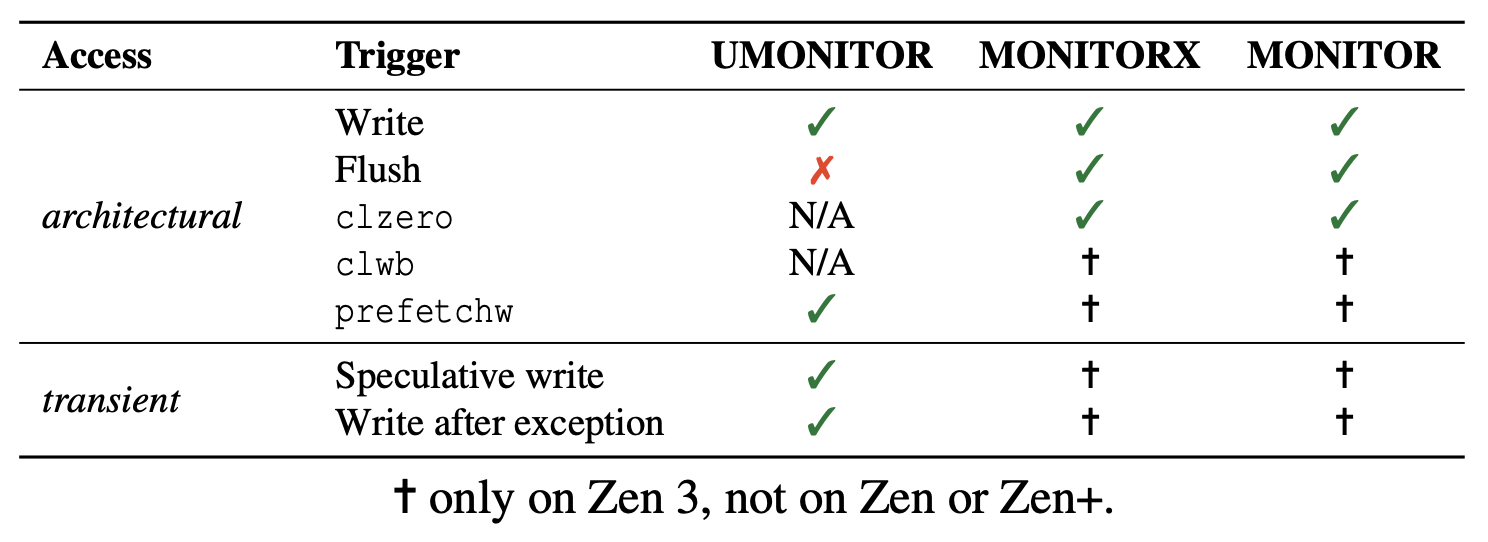
\includegraphics[width=0.6\textwidth]{img/trigger.png}
    \end{center}
\end{figure}
\end{frame}

\begin{frame}{(M)WAIT For it\cite{mwait}}
\begin{figure}
    \begin{center}
    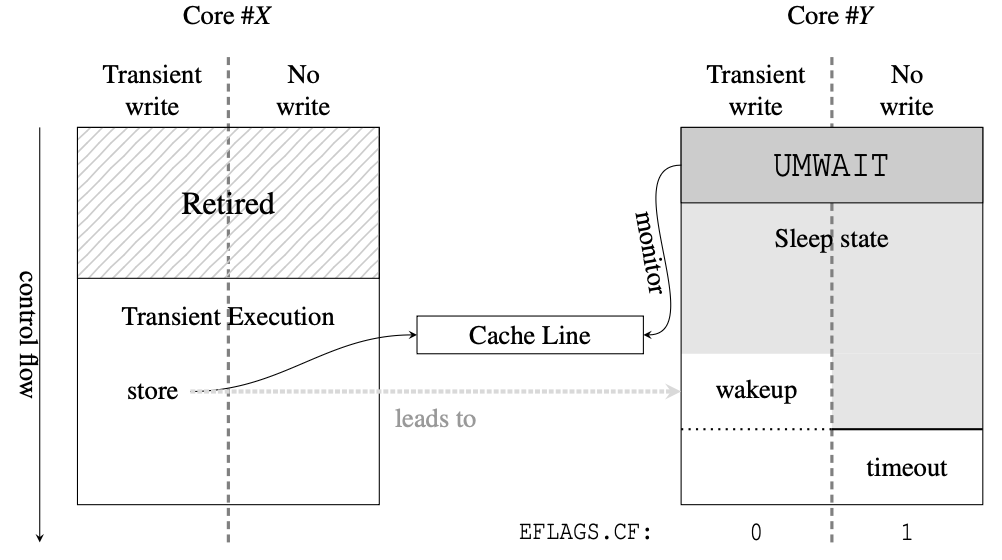
\includegraphics[width=0.6\textwidth]{img/twm.png}
    \end{center}
\end{figure}
\begin{itemize}
    \item Carry flag (CF) is set to 0 if waken up by writing cache/memory, to 1 if waken up due to timeout.
    \item Leaks architectural state about whether the victim transient writes to the target cache line
\end{itemize}
\end{frame}

\begin{frame}{(M)WAIT For it\cite{mwait}}
\begin{figure}
    \begin{center}
    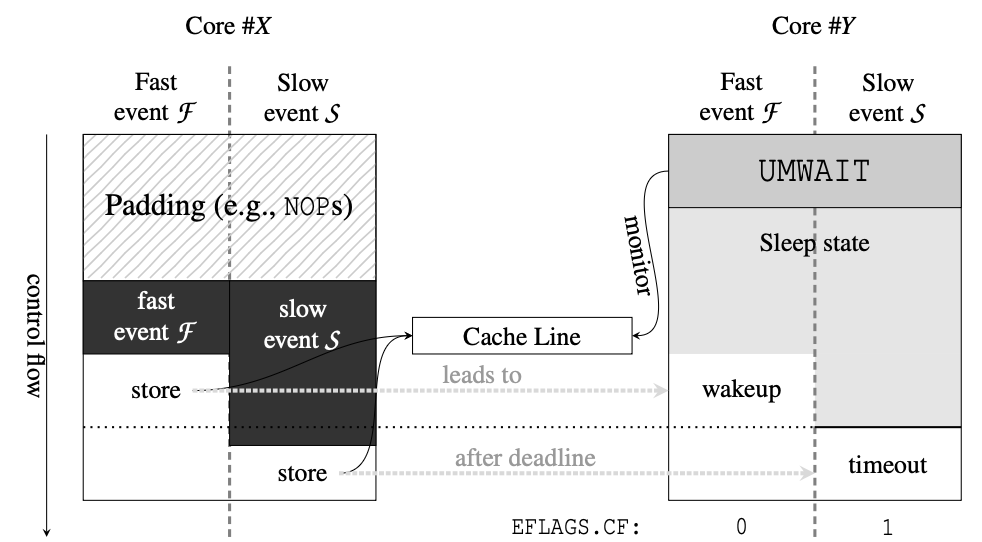
\includegraphics[width=0.7\textwidth]{img/tlt.png}
    \end{center}
\end{figure}
Set a threshold to determine if the targeted memory region is present in cache line $\Rightarrow$ enable a spectre attack without timer.
\end{frame}

\begin{frame}{(M)WAIT For it\cite{mwait}}
Storytelling: build a covert channel to transmit data without a timer.
\begin{figure}
    \begin{center}
    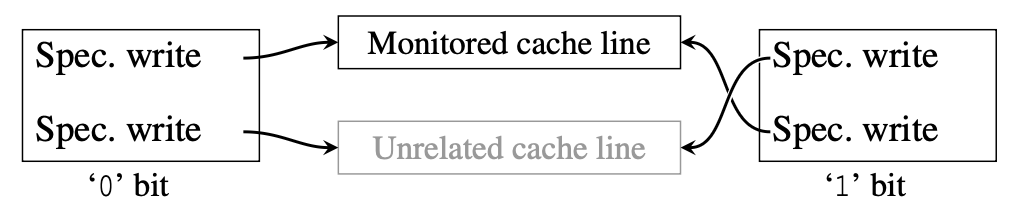
\includegraphics[width=0.9\textwidth]{img/covert.png}
    \end{center}
\end{figure}
\begin{itemize}[<+->]
    \item Carry flag as Manchester-encoded bit to transmit data
    \item An rising edge in CF indicates a 1, a falling edge indicates a 0
    \item Without synchronization, the channel achieves 697 bit/s
\end{itemize}
\end{frame}

\begin{frame}{(M)WAIT For it\cite{mwait}}
Case studies:
\begin{itemize}[<+->]
    \item Spectral: Enhance Spectre PHT with TWM, by monitoring if the target cache line is written without probing the cache line.
    \item Timerless Cache Attacks on OpenSSL 1.0.1 T-Table: Substitute Prime+Probe with TLT.
    \item Network Fingerprints: Utilize \texttt{umwait}'s waken up by external interrupt to fingerprint the network interrupts with a time bucket.
\end{itemize}
\end{frame}

\begin{frame}[allowframebreaks]{References}
\tiny
\printbibliography
\end{frame}
\end{document}
